\subsection{Mechanical/structural design}

For the mechanical design, several factors have been considered to ensure the payload's robustness and easy maintenance:
% \begin{itemize}[leftmargin=1.75cm,itemindent=0cm, noitemsep, topsep=3pt,  label=\faCheck]
%     \item \textbf{Component protection}: The payload's structure has been designed to protect the components from any external impact or shock during the launch and landing;
%     \item \textbf{Resilient structure}: The payload's structure includes shock-absorbing systems such as foam or gel-based layers, springs, or a combination of both. These systems will help to reduce the impact force during landing, preventing damage to the payload and its components;
%     \item \textbf{Easy removal of batteries and radio transmitters}: The batteries and radio transmitters are positioned in a way that allows for easy removal in case of any malfunction or for recharging and testing purposes.;
%     \item \textbf{Easy access to components}: The payload's body has been designed to allow easy extraction of the components for maintenance or replacement in case of malfunctions
%     \item \textbf{Easy removal of batteries and radio transmitter}s: The batteries and radio transmitters are positioned in a way that allows for easy removal in case of any malfunction or for recharging and testing purposes.
% \end{itemize}

\begin{itemize}
    \item \textbf{Component Protection}: The payload's structure will be designed to protect the components from any external impact or shock during the launch and landing.
    \item \textbf{Resilient Structure}: The payload's structure will include some shock-absorbing systems to reduce the impact force during landing, thereby preventing damage to the payload and its components.
    \item \textbf{Easy Removal of Batteries and Radio Transmitters}: The batteries and radio transmitters will be positioned in a way that allows for easy removal in the event of any malfunction, or for recharging and testing purposes.
    \item \textbf{Easy Access to Components}: The design of the payload's body will facilitate easy extraction of the components for maintenance or replacement in case of malfunctions.
\end{itemize}

By taking these factors into account, the team aims to create a robust and reliable payload that can withstand the harsh conditions of the mission and deliver accurate data.

The payload's structure is made from a combination of Polylactic Acid (PLA) and Acrylonitrile Butadiene Styrene (ABS), two lightweight 3D printing materials that provide strength, durability, and exceptional design. This composition allows the can to withstand the stress of launch and landing while maintaining an aerodynamic shape. Additionally, the can is designed with a removable bottom or top section, providing easy access to its internal components. This allows for easy maintenance and repair of the can, without having to dismantle the entire structure.

% Despite PLA's relatively low impact strength, the electronic components housed within the CanSat are protected by 3D-printed supports. The high tensile strength of PLA, which is about 50 MPa, ensures that the 3D-printed parts remain intact when the parachute deploys, preventing disintegration.

The design of the payload is also important to ensure its durability during the launch and landing process. It must withstand high levels of stress and force during these events, so the structure must be designed to distribute and absorb these forces. The can's aerodynamic design is also important for reducing air resistance and achieving maximum altitude during launch.

\begin{table}[htbp]
\centering
\arrayrulecolor{DeepSkyBlue4} % set color of vertical lines
\begin{tabular}{>{\centering\arraybackslash}m{1cm}>{\centering\arraybackslash}lc}
\hline
\rowcolor{DeepSkyBlue4}
&\textbf{\color{white!50}{CanSat Characteristics (description)}} & \textbf{\color{white}{Figure (units)}} \\
\hline
%\rowcolors{2}{LightCyan!50}{}
\adjustbox{valign=m}{
\includegraphics[width=0.6cm]{icons/weight.png}} & Total weight of the payload & 300 g \\
\rowcolor{LightCyan1!50}\adjustbox{valign=m}{
\includegraphics[width=0.5cm]{icons/diameter.png}} & Diameter of the payload & 66 mm\\
\adjustbox{valign=m}{
\includegraphics[width=0.5cm]{icons/recovery.png}} & Length of the recovery system,
including parachute & Max. 60 cm\\
\rowcolor{LightCyan1!50}
\adjustbox{valign=m}{
\includegraphics[width=0.6cm]{icons/time.png}} & Flight time scheduled & 120 s \\
\adjustbox{valign=m}{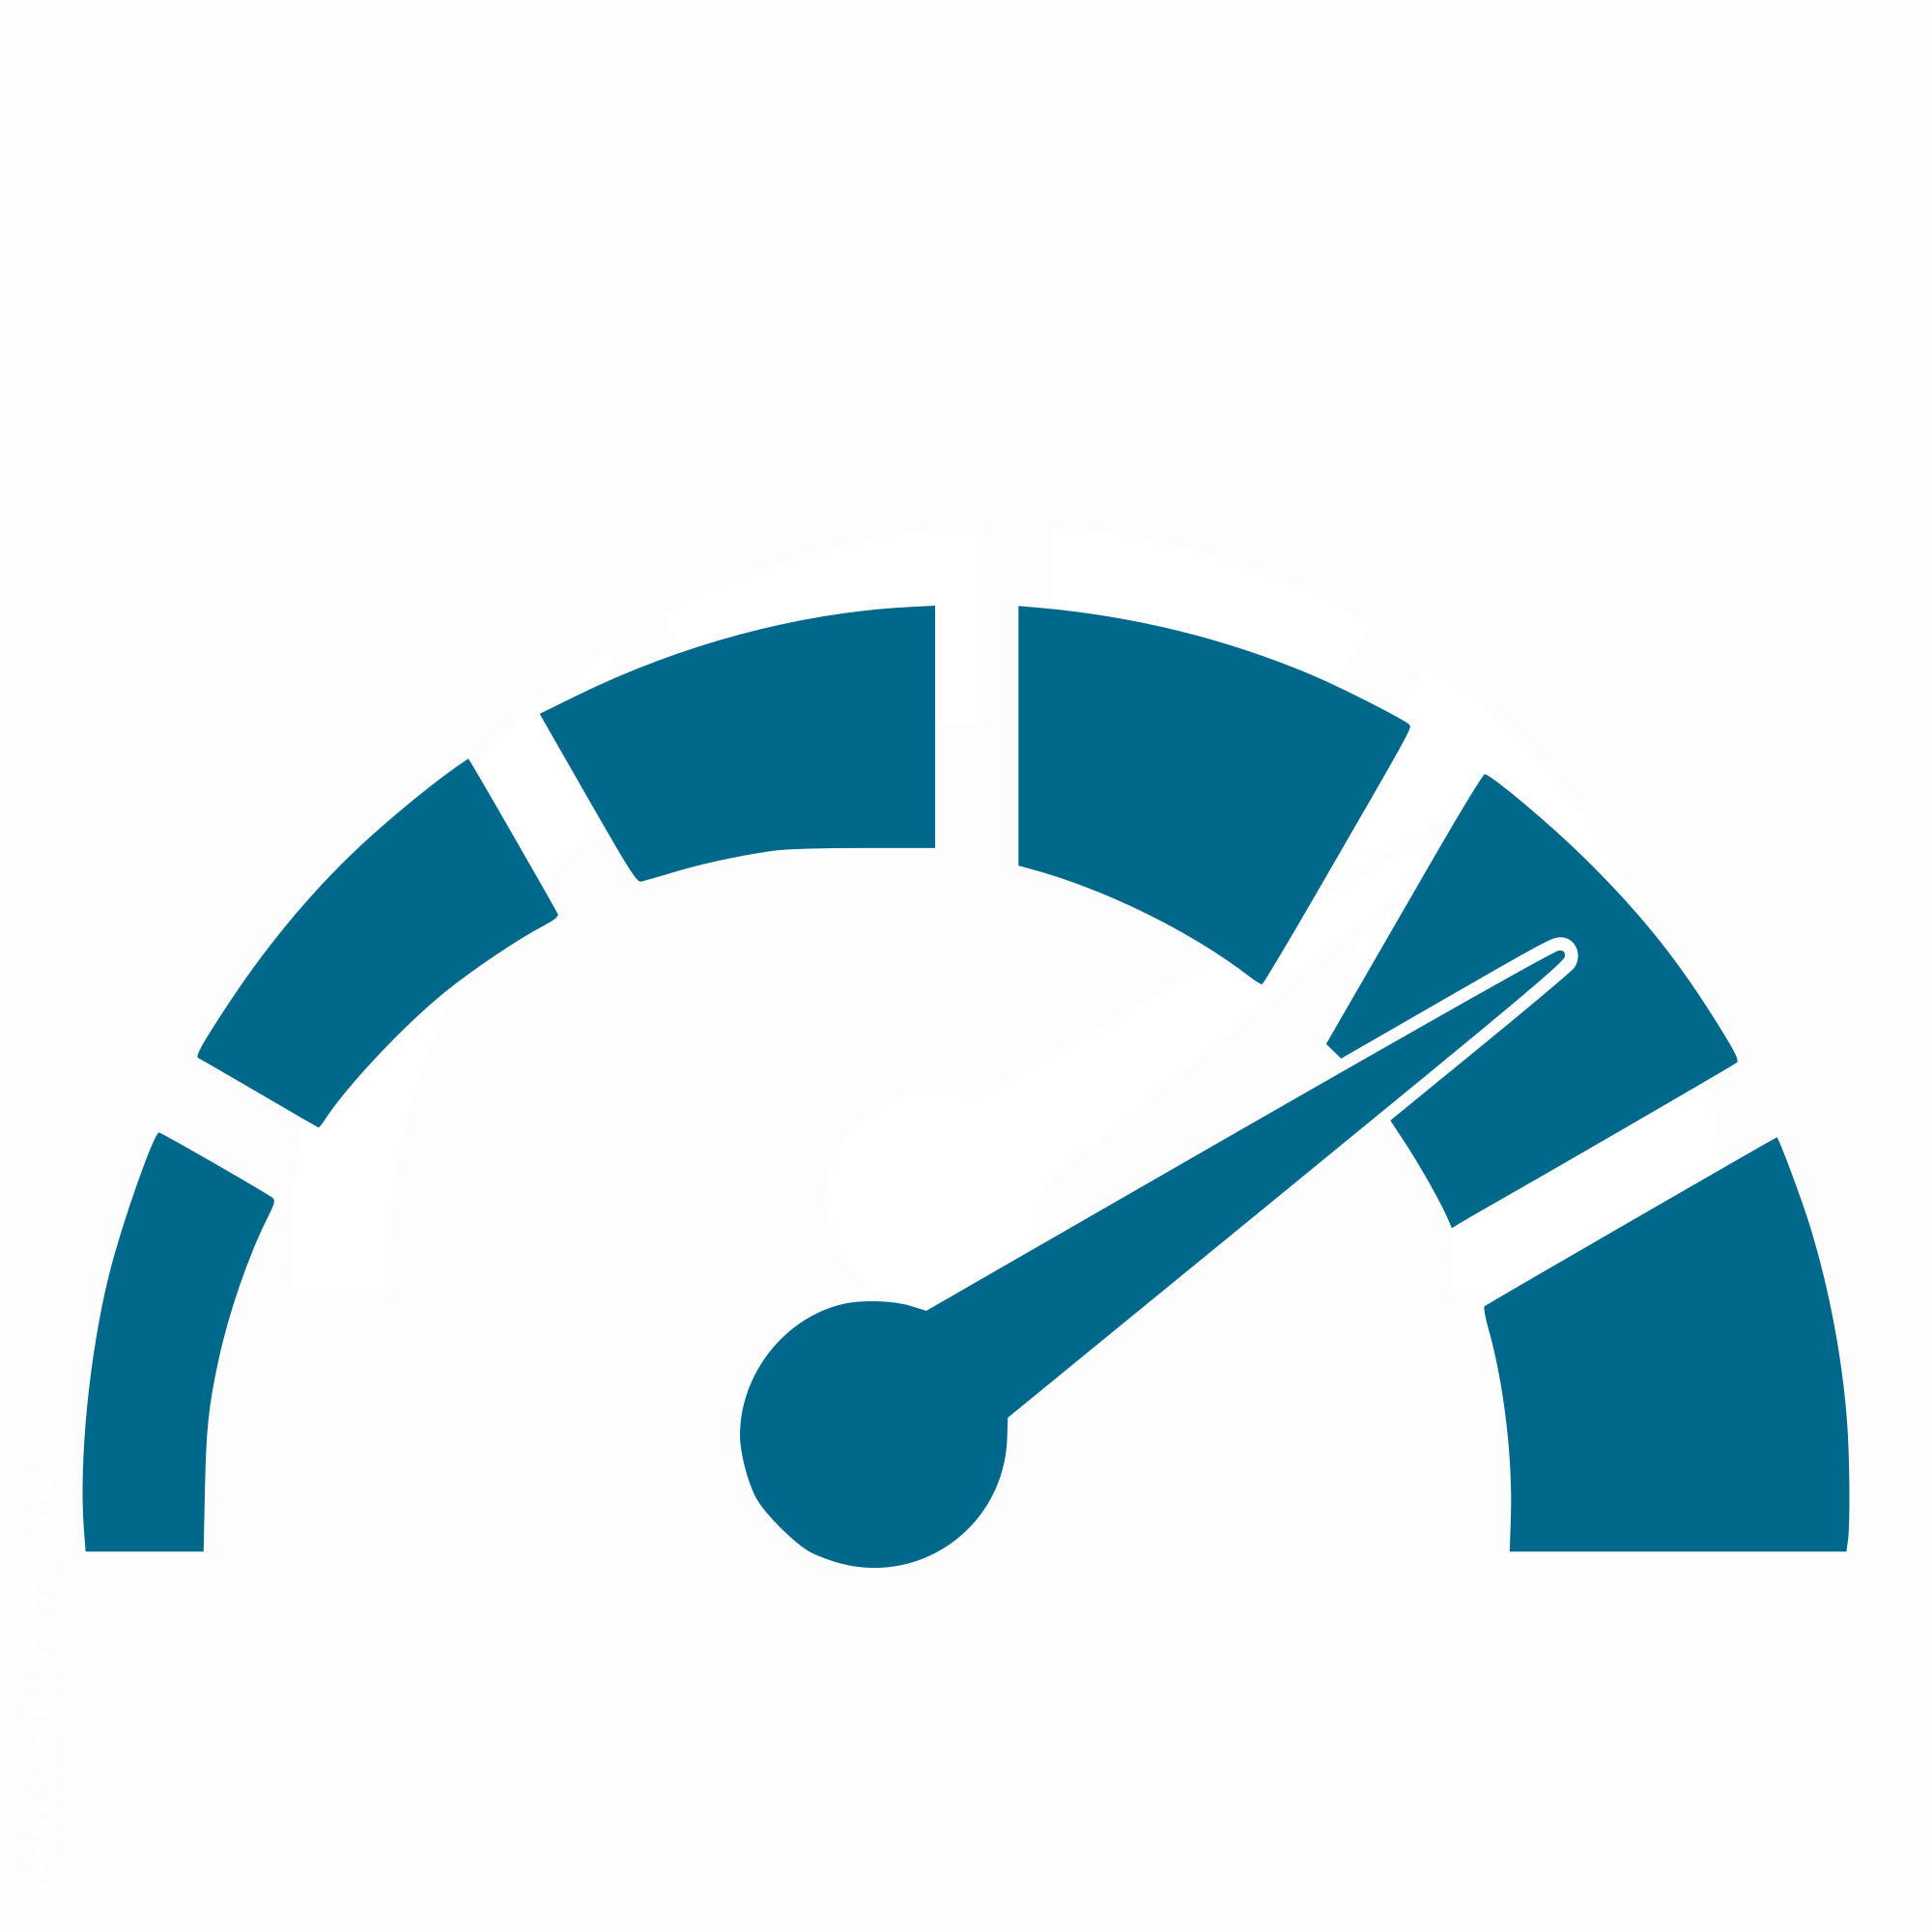
\includegraphics[width=0.6cm]{icons/descent-rate.png}} & Calculated descent rate of the payload & \SI{8 }{\meter\per\second} \\
\rowcolor{LightCyan1!50}
\adjustbox{valign=m}{
\includegraphics[width=0.6cm]{icons/frequency.png}} & Radiofrequency used for
communication & 868 MHz (LoRa) \\
\adjustbox{valign=m}{
\includegraphics[width=0.5cm]{icons/power.png}} & Power consumption of the payload & 450 mA \\
\hline
\end{tabular}
\caption{\small{Main features of the CanSat}}
\end{table}

The payload is composed of several major components, including a few PCB boards that house all the necessary modules. The battery pack, which is the largest and heaviest component, is located at the bottom of the payload and contains pack of four Lithium-Ion battery modules placed in a vertical position. The upper part of the can houses the PCB layers, interconnected with mezzanine connectors, which are fixed in place using screws and glue. % Despite the relatively heavy weight of the battery pack, the can is designed to withstand the stress of launch and landing, and the components are secured in place with 3D-printed supports and foam to prevent damage.

% In order to ensure the functionality of the payload's system during multiple tests, mechanical solutions were explored to protect the can and its contents from the impact of landing. After analyzing various options for shock-absorbing systems, we settled on prototyping and testing the most promising ideas based on their effectiveness, feasibility, and cost. Three potential concepts were identified, including:
% \begin{itemize}[leftmargin=1cm,itemindent=0.5cm, noitemsep, topsep=0pt, label=$\bullet$]
%     \item a foam or gel-based system;
%     \item a spring-based system;
%     \item a combined system using both foam or gel materials and springs.
% \end{itemize}

% The foam or gel-based system involves placing a layer of shock-absorbing foam or gel between two layers of the can, positioned at the bottom opposite to where the parachute is fastened. The spring-based system used a set of springs placed between two bottom layers of the can to compress and absorb the impact of the landing. Finally, the combined system used both springs and foam or gel materials to absorb the initial impact and further reduce the force of the landing, ultimately protecting the CanSat from damage.

The case of the payload will be fitted with inserts on the interior to reinforce its structural strength. To ensure secure closure, the lid is designed to be fastened tightly with screws that fit into specific holes in the cap, requiring a screwdriver to open it. Moreover, the case will have strategically positioned holes to facilitate ideal camera placement and ensure adequate airflow within the can. 
